\section{Question 2: Probability \& Availability}
\textit{Calculate the probability of the top event "Pipeline burst" using the table below. What is the system availability?}
\begin{center}
\line(1,0){250}
\end{center}
\newdimen\nodeDist
\nodeDist=30mm
\newdimen\faillength
\faillength=25mm

\begin{figure}[!ht]
\centering
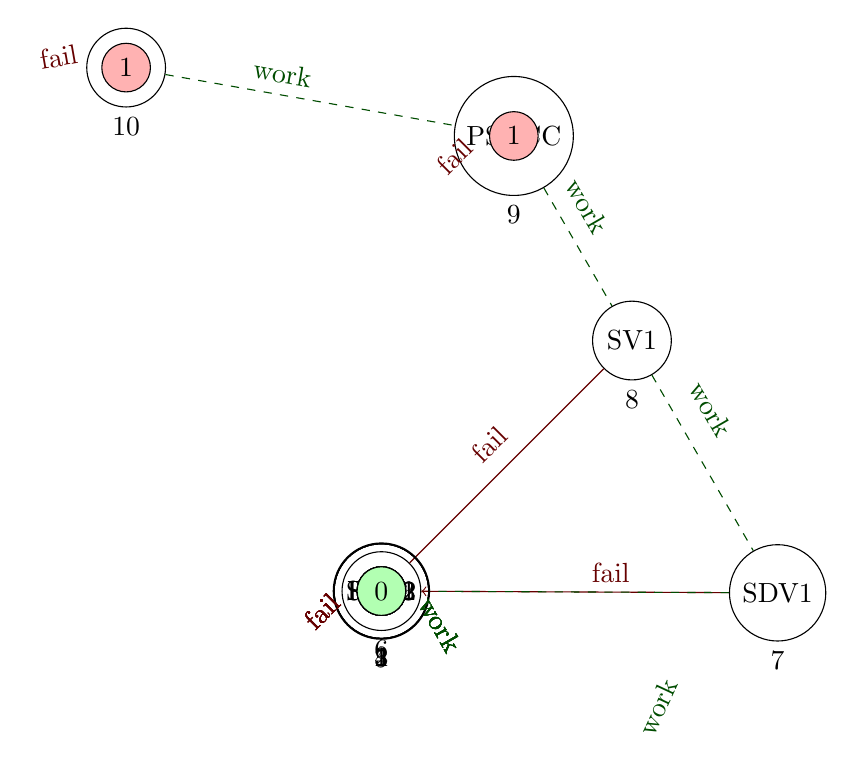
\begin{tikzpicture}[
    node/.style={draw,circle,minimum width=1cm},
    failnode/.style={draw,fill=red!30,circle,minimum width=0.5cm},
    worknode/.style={draw,fill=green!30,circle,minimum width=0.5cm},
]
    \node [label=below:10] [node] (10) {LS};
    \path (10) ++(-170:\faillength) node [failnode] (10l) {1};
    \path (10) ++(-10:50mm) node [label=below:9] [node] (9) {PSHCC};
    \draw [black!60!red] (10) -- (10l) node [yshift=0.2cm,xshift=-0.5cm,rotate=10,left,pos=0] {fail}(10l);
    \draw [dashed, black!70!green] (10) -- (9) node [yshift=0.1cm,xshift=1cm,rotate=-10,right,pos=0] {work}(9);


    \path (9) ++(-135:\faillength) node [failnode] (9l) {1};
    \path (9) ++(-60:30mm) node [label=below:8] [node] (8) {SV1};
    \draw [black!60!red] (9) -- (9l) node [xshift=-0.5cm,rotate=45,left,pos=0] {fail}(9l);
    \draw [dashed, black!70!green] (9) -- (8) node [yshift=0.2cm,xshift=0.3cm,rotate=-60,right,pos=0] {work}(8);
    
    \path (8) ++(-135:45mm) node [label=below:6] [node] (6) {SV2};
    \path (8) ++(-60:37mm) node [label=below:7] [node] (7) {SDV1};
    \draw [black!60!red] (8) -- (6) node [yshift=-0.7cm,xshift=-1.2cm,rotate=45,left,pos=0] {fail}(6);
    \draw [dashed, black!70!green] (8) -- (7) node [xshift=0.5cm,rotate=-60,right,pos=0] {work}(7);
    \draw [black!60!red,->] (7) -- (6) node [xshift=-1.5cm,rotate=0,above,pos=0] {fail}(6);


   \path (6) ++(-135:\faillength) node [failnode] (6l) {1};
    \path (6) ++(-60:\nodeDist) node [label=below:5] [node] (5) {SDV2};
    \draw [black!60!red] (6) -- (6l) node [xshift=-0.5cm,rotate=45,left,pos=0] {fail}(6l);
    \draw [dashed, black!70!green] (6) -- (5) node [xshift=0.5cm,rotate=-60,right,pos=0] {work}(5);
    

   \path (5) ++(-135:\faillength) node [failnode] (5l) {1};
    \path (5) ++(-60:\nodeDist) node [label=below:4] [node] (4) {PSH1};
    \draw [black!60!red] (5) -- (5l) node [xshift=-0.5cm,rotate=45,left,pos=0] {fail}(5l);
    \draw [dashed, black!70!green] (5) -- (4) node [xshift=0.5cm,rotate=-60,right,pos=0] {work}(4);
    
\draw [dashed, black!70!green] (7) -- (4) node [yshift=-1cm,xshift=-0.7cm,rotate=65,left,pos=0] {work}(4);
    
    
    \path (4) ++(-135:\nodeDist) node [label=below:3] [node] (3) {PSH2};
    \path (4) ++(-60:\nodeDist) node [label=below:2] [node] (2) {PSH2};
    \draw [black!60!red] (4) -- (3) node [xshift=-0.5cm,rotate=45,left,pos=0] {fail}(3);
    \draw [dashed, black!70!green] (4) -- (2) node [xshift=0.5cm,rotate=-60,right,pos=0] {work}(2);


    \path (2) ++(-135:\nodeDist) node [label=below:1] [node] (1) {PSH3};
    \path (3) ++(-135:\nodeDist) node [failnode] (3l) {1};
    \path (2) ++(-60:\nodeDist) node [worknode] (2r) {0};
    
    \draw [black!60!red] (3) -- (3l) node [xshift=-0.5cm,rotate=45,left,pos=0] {fail}(3l);
    \draw [black!60!red] (2) -- (1) node [xshift=-0.5cm,rotate=45,left,pos=0] {fail}(1);
    \draw [dashed, black!70!green] (3) -- (1) node [xshift=0.5cm,rotate=-60,right,pos=0] {work}(1);
    \draw [dashed, black!70!green] (2) -- (2r) node [xshift=0.5cm,rotate=-60,right,pos=0] {work}(2r);
    
    \path (1) ++(-135:\nodeDist) node [failnode] (1l) {1};
    \path (1) ++(-60:\nodeDist) node [worknode] (1r) {0};

    \draw [black!60!red] (1) -- (1l) node [xshift=-0.5cm,rotate=45,left,pos=0] {fail}(1l);
    \draw [dashed, black!70!green] (1) -- (1r) node [xshift=0.5cm,rotate=-60,right,pos=0] {work}(1r);

\end{tikzpicture}
\caption{Decision tree for probabiability calculation}\label{fig:decisiontree}
\end{figure}

To calculate the probability for the TOP event it is not sufficient to use the approximation of summing up the probabilities of the minimal cutsets. A decision tree (See figure \ref{fig:decisiontree}) has been used to calculate the probability while disjointing the cutsets.

\begin{table}[!ht]
\centering
\renewcommand{\arraystretch}{1.4}
\label{tab:events}
\begin{tabular}{|l|l|l|l|l|}
\hline
\textbf{Basic Event}                       & \textbf{Abbreviation} & \textbf{Distribution}        & \textbf{Symbol}       & \textbf{Value}      \\ \hline
Pressure Sensor 1 Failure             & PSH1                      & \multirow{3}{*}{Exponential}                  & \multirow{3}{*}{$\lambda_{PSH}$}    & \multirow{3}{*}{$7\times10^{-7}$}  \\ \cline{1-2}
Pressure Sensor 2 Failure             & PSH2                      &                              &                       &                     \\ \cline{1-2}
Pressure Sensor 3 Failure             & PSH3                      &                              &                       &                     \\ \hline
Pressure Sensor Common Cause Failure & PSHCC                     & Exponential                  & $\lambda_{PSHCC}$                     & $3,5\times10^{-8}$                  \\ \hline
Solenoid Valve 1 Failure             & SV1                       & \multirow{2}{*}{Exponential} &  \multirow{2}{*}{$\lambda_{SV}$}   & \multirow{2}{*}{$2,6\times10^{-6}$} \\ \cline{1-2}
Solenoid Valve 2 Failure             & SV2                       &                              &                       &                     \\ \hline
Shutdown Valve 1 Failure             & SDV1                      & \multirow{2}{*}{Exponential} &  \multirow{2}{*}{$\lambda_{SDV}$} & \multirow{2}{*}{$4,1\times10^{-6}$} \\ \cline{1-2}
Shutdown Valve 2 Failure             & SDV2                      &                              &                       &                     \\ \hline
Logic Solver Failure                 & LS                        & GLM                          &  $\lambda_{LS}$                     & $1\times10^{-6}$                   \\ \hline
Logic Solver Repair                 & -                        & Exponential                          &  $\mu_{LS}$                     & $0,1$                   \\ \hline
\end{tabular}
\caption{Tabular overview of possible events, their name, symbol and failure rate}
\end{table}

Table \ref{tab:events} lists all given basic events, their failure rate and their abbreviated name. Furthermore the symbol chosen is shown. The Logic Solver failure rate distribution is assumed to follow the exponential distribution law as soon as it is in operation.

\begin{table}[!ht]
\centering
\renewcommand{\arraystretch}{1.4}
\label{tab:probcalculation}
\begin{tabular}{|l|l|}
\hline
\textbf{Node No.} & \textbf{Calculation}  \\ \hline
Node 10           & p(LS)*1+(1-p(LS))*p(N9)                \\ \hline
Node 9            & p(PSHCC)*1+(1-p(PSHCC))*p(N8)         \\ \hline
Node 8            & p(SV1)*p(N6) + (1-p(SV1))*p(N7)         \\ \hline
Node 7            & p(SDV1)*p(N6) + (1-p(SDV1))*p(N4)     \\ \hline
Node 6            & p(SV2)*1 + (1-p(SV2))*p(N5)         \\ \hline
Node 5            & p(SDV2)*1+(1-p(SDV2))*p(N4)        \\ \hline
Node 4            & p(PSH1)*p(N3) + (1-p(PSH1))*p(N2)      \\ \hline
Node 3            & p(PSH2)*1 + (1-p(PSH2))*p(N1)       \\ \hline
Node 2            & p(PSH2)*p(N1) + (1-p(PSH2))*0       \\ \hline
Node 1            & p(PSH3)*1 + (1-p(PSH3))*0      \\ \hline
\end{tabular}
\caption{Calculation of probability with decision tree}
\end{table}

The reliability function for each of the nodes is $R(t) = e^{- \lambda\times t}$. These equations have been calculated cascading to get the reliability for the top node 10. The used $t$ is ranging from 0 (the start) to 5.000.000 hours. The MTTF for items following the exponential law for failure distribution is calculated by $MTTF = \frac{1}{\lambda}$. Table \ref{tab:mttf} shows the calculated MTTF values for all items.

\begin{table}[!ht]
\centering
\renewcommand{\arraystretch}{1.4}
\label{tab:mttf}
\begin{tabular}{|l|l|l|}
\hline
\textbf{Basic Event}                  & \textbf{Abbreviation} & \textbf{MTTF [h]}         \\ \hline
Pressure Sensor 1 Failure             & PSH1                      & 1.428.571                   \\\hline
Pressure Sensor 2 Failure             & PSH2                      &  1.428.571      \\ \hline
Pressure Sensor 3 Failure             & PSH3                      &   1.428.571            \\ \hline
Pressure Sensor Common Cause Failure & PSHCC                     &   28.571.429          \\ \hline
Solenoid Valve 1 Failure             & SV1                       & 384.616 \\ \hline
Solenoid Valve 2 Failure             & SV2                       &  384.616 \\ \hline
Shutdown Valve 1 Failure             & SDV1                      & 243.903\\ \hline
Shutdown Valve 2 Failure             & SDV2                      & 243.903    \\ \hline
Logic Solver Failure                 & LS                        & 1.000.000           \\ \hline
\end{tabular}
\caption{Tabular overview of the calculated MTTF}
\end{table}


\begin{figure}[!ht]
\centering
\begin{tikzpicture}
\begin{axis}[
    %title={Temperature dependence of CuSO$_4\cdot$5H$_2$O solubility},
    xlabel={Time [1000 hours]},
    %ylabel={Solubility [g per 100 g water]},
    xmin=0, xmax=5000,
    ymin=0, ymax=1,
%    xtick={0,20,40,60,80,100},
%    ytick={0,20,40,60,80,100,120},
    legend pos=north east,
    ymajorgrids=true,
    grid style=dashed,
]
 
\addplot[
    color=blue,
    %mark=square,
    name path=A
    ]
    coordinates {
    (50,0.9966082939)(100,0.9874435882)(200,0.9566302805)(300,0.9148991942)(400,0.8668784542)(500,0.8155217682)(600,0.762750925)(700,0.7098497403)(800,0.6577020106)(900,0.60693306)(1000,0.5579931101)(1100,0.5112065293)(1200,0.4668016816)(1300,0.4249300835)(1400,0.3856798361)(1500,0.3490860317)(1600,0.3151395245)(1700,0.2837947132)(1800,0.2549765994)(1900,0.2285871977)(2000,0.2045112978)(2100,0.1826215595)(2200,0.1627829335)(2300,0.1448564154)(2400,0.1287021628)(2500,0.114182018)(2600,0.1011614925)(2700,0.0895112752)(2800,0.0791083252)(2900,0.069836614)(3000,0.0615875745)(3100,0.0542603114)(3200,0.0477616212)(3300,0.0420058631)(3400,0.0369147192)(3500,0.0324168726)(3600,0.0284476301)(3700,0.0249485094)(3800,0.021866808)(3900,0.0191551671)(4000,0.0167711393)(4100,0.0146767688)(4200,0.0128381894)(4300,0.0112252431)(4400,0.0098111223)(4500,0.0085720375)(4600,0.0074869093)(4700,0.0065370858)(4800,0.0057060845)(4900,0.0049793571)(5000,0.0043440766)
    };
    \legend{Availability}
    
\addplot[
    color=red,
    name path=U,
    ]
    coordinates {
    (50,0.0033917061)(100,0.0125564118)(200,0.0433697195)(300,0.0851008058)(400,0.1331215458)(500,0.1844782318)(600,0.237249075)(700,0.2901502597)(800,0.3422979894)(900,0.39306694)(1000,0.4420068899)(1100,0.4887934707)(1200,0.5331983184)(1300,0.5750699165)(1400,0.6143201639)(1500,0.6509139683)(1600,0.6848604755)(1700,0.7162052868)(1800,0.7450234006)(1900,0.7714128023)(2000,0.7954887022)(2100,0.8173784405)(2200,0.8372170665)(2300,0.8551435846)(2400,0.8712978372)(2500,0.885817982)(2600,0.8988385075)(2700,0.9104887248)(2800,0.9208916748)(2900,0.930163386)(3000,0.9384124255)(3100,0.9457396886)(3200,0.9522383788)(3300,0.9579941369)(3400,0.9630852808)(3500,0.9675831274)(3600,0.9715523699)(3700,0.9750514906)(3800,0.978133192)(3900,0.9808448329)(4000,0.9832288607)(4100,0.9853232312)(4200,0.9871618106)(4300,0.9887747569)(4400,0.9901888777)(4500,0.9914279625)(4600,0.9925130907)(4700,0.9934629142)(4800,0.9942939155)(4900,0.9950206429)(5000,0.9956559234)
%    coordinates {
%    (0,0)(4000,0.5)
    };
    \addlegendentry{Unavailability}
\end{axis}
\end{tikzpicture}
\caption{Development of Availability and Reliability}\label{fig:graph}
\end{figure}
